\documentclass[article,12pt]{elsarticle}
\usepackage[utf8]{inputenc}
\usepackage{graphicx}
\usepackage{booktabs}
\usepackage{subcaption}
\usepackage{amssymb}
\usepackage{flushend}
\usepackage{float}
\usepackage{amsmath}
\usepackage{amsfonts}
\usepackage{dcolumn}
\usepackage{amsthm}
\usepackage{caption}
\usepackage{lmodern}
\usepackage{booktabs}
\usepackage{color}
\usepackage{longtable}
\usepackage{rotating}
\usepackage{etoolbox}
\usepackage{hyperref}
\usepackage{comment}
\usepackage{pdflscape}
\usepackage{comment}
\usepackage{xcolor}  % <- Este paquete permite usar colores en tablas
\usepackage{colortbl} % <- Para colorear celdas en tablas
\usepackage[table,xcdraw]{xcolor}
\usepackage[framemethod=TikZ]{mdframed}
\usepackage[a4paper, left=1.5cm, right=1.5cm, top=2cm, bottom=2cm]{geometry}

\begin{document}

\mdfsetup{innertopmargin=10pt,linecolor=blue!20,%
linewidth=2pt,topline=true,
frametitleaboveskip=\dimexpr-\ht\strutbox\relax,}

\begin{frontmatter}
    \title{Laboratorio de Óptica \\  Práctica  III: Espejos}
    \author{López González Andrés$^1$, Reyes Saldivar Ailton Uriel$^2$ y Gante Morales Pedro José$^3$} %Aquí va el nombre de los integrantes que participaron en el informe.
    \address{$^1$ Facultad de Ciencias, Universidad Nacional Autónoma de México, M\'exico CDMX.}

\begin{abstract}

En este experimento se analizaron las propiedades de los espejos planos y esféricos a través de diversas mediciones y comprobaciones experimentales. Se verificó la ecuación del espejo plano mediante triangulación, observando que la distancia imagen coincide con la distancia objeto. Asimismo, se midió el radio de curvatura de un espejo cóncavo utilizando un esferómetro y la ecuación del espejo, comparando ambos resultados. Además, se estudió la formación de imágenes en espejos cóncavos al variar la posición del objeto y se comprobó la ecuación de magnificación. Los resultados obtenidos permiten validar los principios de la óptica geométrica y su aplicación en la caracterización de sistemas ópticos.


\end{abstract}
    
\end{frontmatter}

\vspace{0.5cm} 

\section{Introducción}

La óptica geométrica estudia el comportamiento de la luz al interactuar con diferentes superficies reflectantes y refractantes. Entre los dispositivos ópticos más fundamentales se encuentran los espejos, cuya capacidad de reflejar la luz se basa en la Ley de la Reflexión \cite{Pedrotti2018, Hecht2000}. Dependiendo de la forma de la superficie reflectante, los espejos pueden clasificarse en planos y esféricos, y su aplicación varía desde el uso en instrumentos científicos hasta objetos cotidianos como retrovisores y telescopios \cite{Tipler1999}.

El estudio de los espejos es relevante en diversas áreas de la física y la ingeniería óptica, ya que permiten la manipulación de la trayectoria de los rayos de luz para generar imágenes con características específicas. Las imágenes formadas por los espejos pueden ser reales o virtuales, dependiendo de la posición del objeto y la geometría del espejo \cite{Serway2002}.

\subsection{Espejos Planos}
Los espejos planos son superficies reflectantes sin curvatura. La imagen de un objeto colocado frente a un espejo plano aparece a la misma distancia detrás del espejo, cumpliendo la relación:

\begin{mdframed}
\begin{equation}
    o = i
\end{equation}
\end{mdframed}
donde $o$ es la distancia del objeto al espejo y $i$ la distancia de la imagen. La imagen es virtual, derecha e idéntica en tamaño al objeto \cite{Pedrotti2018}.

Estos espejos son ampliamente utilizados en la vida cotidiana, como en los espejos domésticos y en sistemas ópticos donde se requiere una reflexión sin distorsión. Dado que los espejos planos producen imágenes virtuales, no pueden proyectarse en una pantalla, ya que los rayos reflejados parecen provenir de un punto detrás del espejo sin realmente converger en él.

\subsection{Espejos Esféricos}
Los espejos esféricos poseen una curvatura que modifica el comportamiento de la luz reflejada, permitiendo la formación de imágenes con distintas características según la posición del objeto. Se dividen en dos tipos:
\begin{itemize}
    \item \textbf{Cóncavos}: La superficie reflectante está en la cara interna de la esfera. Estos espejos pueden formar imágenes reales o virtuales dependiendo de la posición del objeto. Son utilizados en telescopios, reflectores y dispositivos ópticos que requieren la concentración de la luz \cite{Hecht2000}.
    \item \textbf{Convexos}: La superficie reflectante está en la cara externa. Siempre generan imágenes virtuales, menores y derechas. Son comunes en espejos de seguridad y retrovisores, ya que permiten un amplio campo de visión \cite{Tipler1999}.
\end{itemize}

Para determinar la posición de la imagen en espejos esféricos, se utiliza la ecuación del espejo:

\begin{mdframed}
\begin{equation}
    \frac{1}{o} + \frac{1}{i} = \frac{2}{R}
\end{equation}
\end{mdframed}
\begin{mdframed}
donde $R$ es el radio de curvatura del espejo. En términos del foco $f = \frac{R}{2}$, la ecuación se reescribe como:
\begin{equation}
    \frac{1}{o} + \frac{1}{i} = \frac{1}{f}
\end{equation}
\end{mdframed}

La magnificación lateral de la imagen está dada por:

\begin{mdframed}
\begin{equation}
    M = -\frac{i}{o} = \frac{h'}{h}
\end{equation}
\end{mdframed}
donde $h$ y $h'$ son las alturas del objeto y de la imagen, respectivamente. La magnificación determina si la imagen es aumentada o reducida y si es invertida o derecha \cite{Serway2002}.

\subsection{Esferómetro}
El esferómetro es un instrumento para medir el radio de curvatura de superficies esféricas. Su diseño consta de un tornillo micrométrico montado sobre un trípode equilátero, permitiendo la medición precisa de la altura de una superficie curva. Se basa en la relación geométrica:

\begin{mdframed}
\begin{equation}
    R = \frac{a^2}{2h} + \frac{h}{2}
\end{equation}
\end{mdframed}

donde $a$ es la distancia entre patas del esferómetro y $h$ la altura medida por el tornillo micrométrico \cite{Khan2015}.

El uso del esferómetro es fundamental en la óptica, ya que permite conocer el radio de curvatura de espejos y lentes, lo cual es esencial para el diseño y calibración de sistemas ópticos de precisión.

\subsection{Linealización de la ecuación del espejo}
La ecuación del espejo esférico es:

\begin{mdframed}
\begin{equation}
    \frac{1}{o} + \frac{1}{i} = \frac{2}{R}
\end{equation}
\end{mdframed}

Donde:
\begin{itemize}
    \item $o$ es la distancia del objeto al espejo.
    \item $i$ es la distancia de la imagen al espejo.
    \item $R$ es el radio de curvatura del espejo.
\end{itemize}
Para linealizar esta ecuación, la reescribimos como:
\begin{mdframed}
\begin{equation}
    \frac{1}{i} = \frac{2}{R} - \frac{1}{o}
\end{equation}
\end{mdframed}
Definiendo las variables:

\begin{mdframed}
\begin{equation}
    x' = \frac{1}{o}, \quad y' = \frac{1}{i}
\end{equation}
\end{mdframed}

La ecuación toma la forma de una ecuación de una recta:
\begin{mdframed}
\begin{equation}
    y' = -x' + \frac{2}{R}
\end{equation}
\end{mdframed}
Comparándola con la ecuación general de la recta $y = mx + b$, identificamos:
\begin{itemize}
    \item $x' = \frac{1}{o}$ (variable independiente)
    \item $y' = \frac{1}{i}$ (variable dependiente)
    \item $m = -1$ (pendiente)
    \item $b = \frac{2}{R}$ (ordenada al origen)
\end{itemize}




\subsection{Hipótesis}

Dado que la formación de imágenes en espejos se rige por relaciones matemáticas bien establecidas, se espera que:
\begin{itemize}
    \item La distancia de la imagen en un espejo plano sea igual a la distancia del objeto ($i = o$), lo cual se verificará mediante triangulación en una hoja milimétrica.
    \item La medición del radio de curvatura con el esferómetro sea consistente con la obtenida mediante la linealización de la ecuación del espejo ($R = 2/b$).
    \item La ecuación de magnificación obtenida con las distancias ($M = -i/o$) coincida con la obtenida mediante la comparación de tamaños de imagen y objeto ($M = h_i/h_o$).
\end{itemize}


\subsection{Objetivos}

Los objetivos de este informe son:
\begin{itemize}
    \item Verificar experimentalmente la ecuación del espejo plano mediante la comparación de distancias del objeto e imagen.
    \item Determinar el radio de curvatura de un espejo esférico utilizando dos métodos: el esferómetro y la linealización de la ecuación del espejo.
    \item Evaluar la relación entre la magnificación calculada a partir de las distancias del objeto e imagen y la obtenida mediante la comparación de alturas.
    \item Analizar la propagación de incertidumbre en la determinación del radio de curvatura, la distancia focal y la magnificación.
\end{itemize}


\section{Desarrollo Experimental}
\subsection{Determinación de la Distancia Imagen en un Espejo Plano}
Para esta parte del experimento, se utilizó un espejo plano colocado sobre una hoja cuadriculada. El procedimiento seguido fue el siguiente:

\begin{enumerate}
    \item Se dibujó un sistema de coordenadas en la hoja cuadriculada, donde el eje $x$ coincidió con la base del espejo y el eje $y$ representó la distancia objeto-imagen.
    \item Se colocó un objeto en un punto determinado sobre el eje $y$ y se registró su distancia con respecto al espejo.
    \item Mediante el método de triangulación, se marcaron tres líneas de observación con la ayuda de una regla, considerando diferentes ángulos de visión del objeto reflejado en el espejo.
    \item Se trazaron las prolongaciones de estas líneas hasta su intersección, la cual corresponde a la posición esperada de la imagen virtual del objeto.
    \item Se midió la distancia desde el espejo hasta la intersección de las líneas para determinar la distancia imagen y se comparó con la distancia objeto.
\end{enumerate}

De acuerdo con la teoría de los espejos planos, la distancia imagen debe ser igual a la distancia objeto, verificando así la ecuación $o = i$. Esta comprobación experimental permitió validar la ley de reflexión en espejos planos.

\begin{figure}[H]
    \centering
    \begin{minipage}{0.30\textwidth}
        \centering
        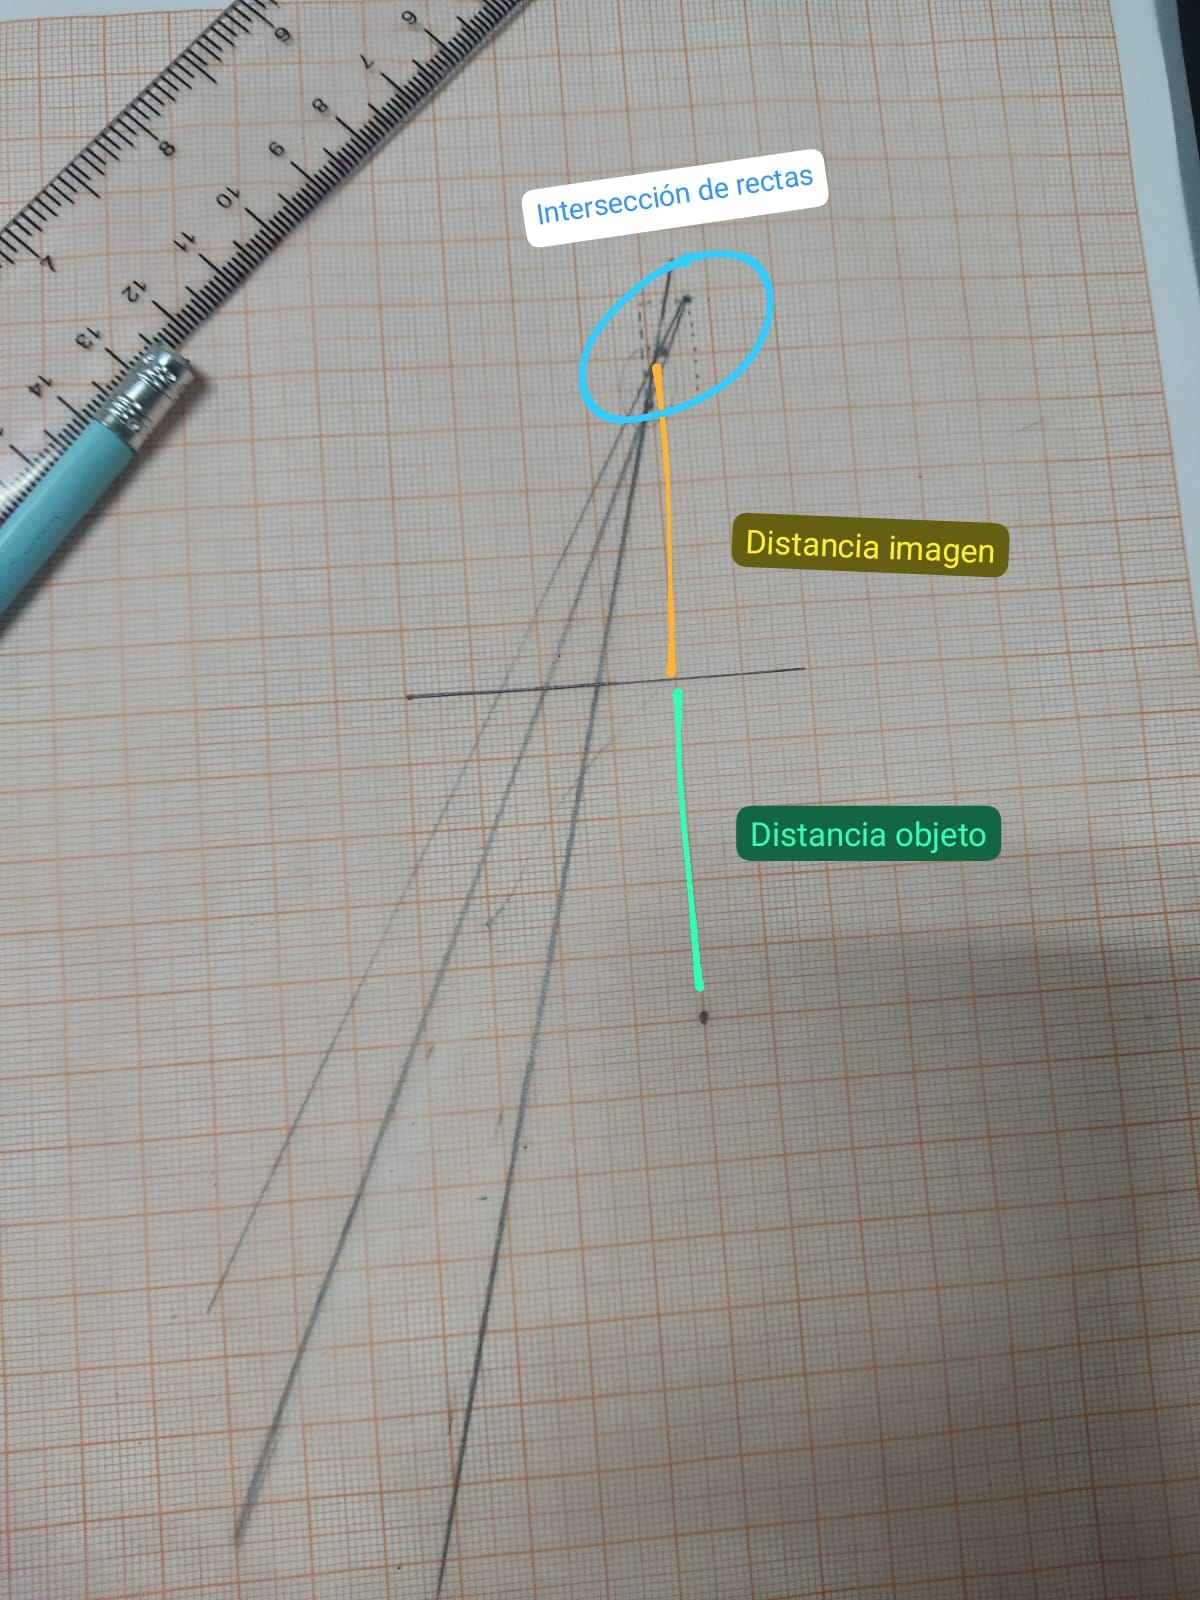
\includegraphics[width=\textwidth]{espejo plano arreglo 1.jpeg}
        \caption{Arreglo experimental del espejo plano}
        \label{fig:imagen1}
    \end{minipage}
    \hfill
    \begin{minipage}{0.30\textwidth}
        \centering
        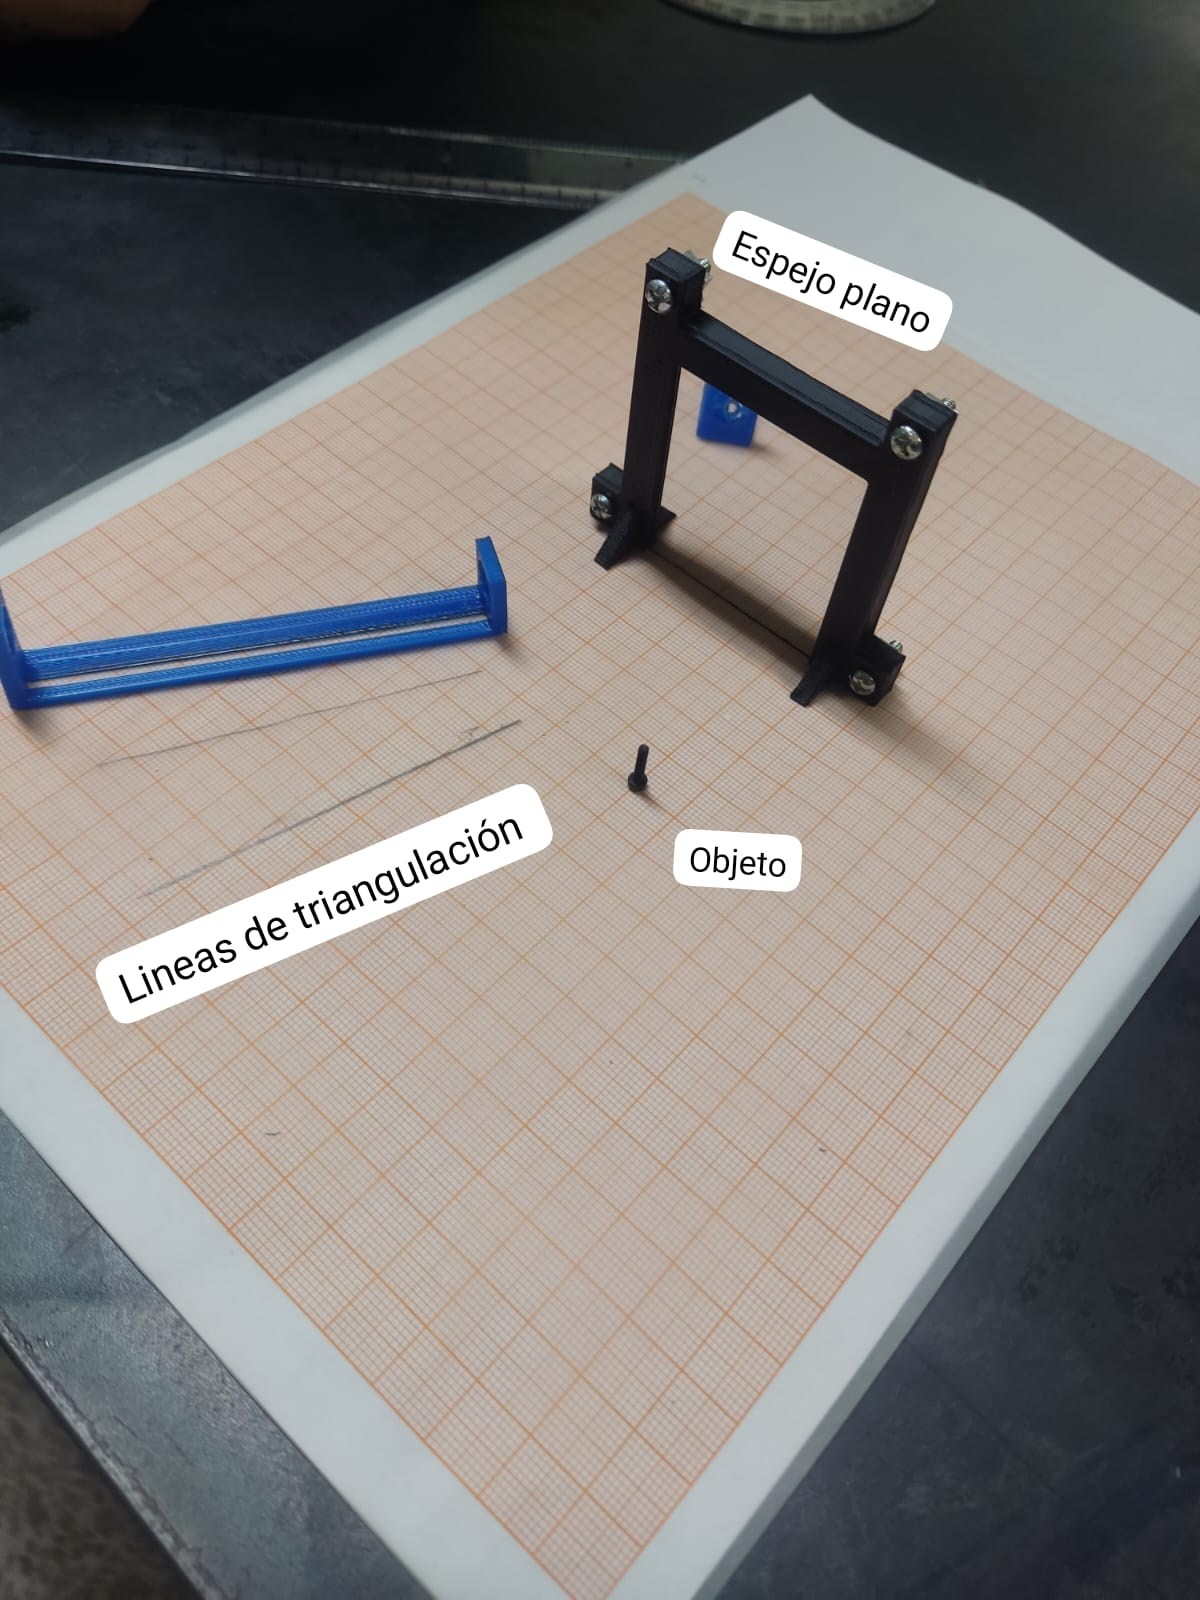
\includegraphics[width=\textwidth]{esoejo plano arreglo 2.jpeg}
        \caption{Resultado de la triangulación}
        \label{fig:imagen2}
    \end{minipage}
\end{figure}

\subsection{Calculo del radio de curvatura del espejo cóncavo con un esferómetro}

\begin{enumerate}
    \item Se midió el radio del esferómetro ($a$) utilizando un vernier, obteniendo $a = 18.00 \pm 0.05$ mm.
    \item El esferómetro cuenta con un tornillo micrométrico que se puede desplazar verticalmente al girarlo. Este tornillo está incrustado en el centro de un anillo que define un plano de referencia.
    \item La escala del esferómetro tiene una resolución mínima de $0.01$ mm, y cada vuelta completa del tornillo equivale a un desplazamiento vertical de $0.5$ mm. La escala está dividida en cuatro partes.
    \item Se calibró el esferómetro colocándolo sobre una superficie plana y girando el tornillo levemente hasta que dejó de moverse. Este punto se estableció como el cero de referencia.
    \item Luego, se colocó el esferómetro sobre la superficie del espejo esférico cóncavo y se giró el tornillo micrométrico hasta que tocó la superficie del espejo.
    \item Se midió el desplazamiento vertical ($h$), considerando el número de vueltas del tornillo y la resolución del dispositivo.
    \item Con los valores de $a$ y $h$, se calculó el radio de curvatura del espejo utilizando la ecuación:
    \begin{equation}
        R = \frac{a^2}{2h} + \frac{h}{2}
    \end{equation}
\end{enumerate}

\begin{figure}[H]
    \centering
    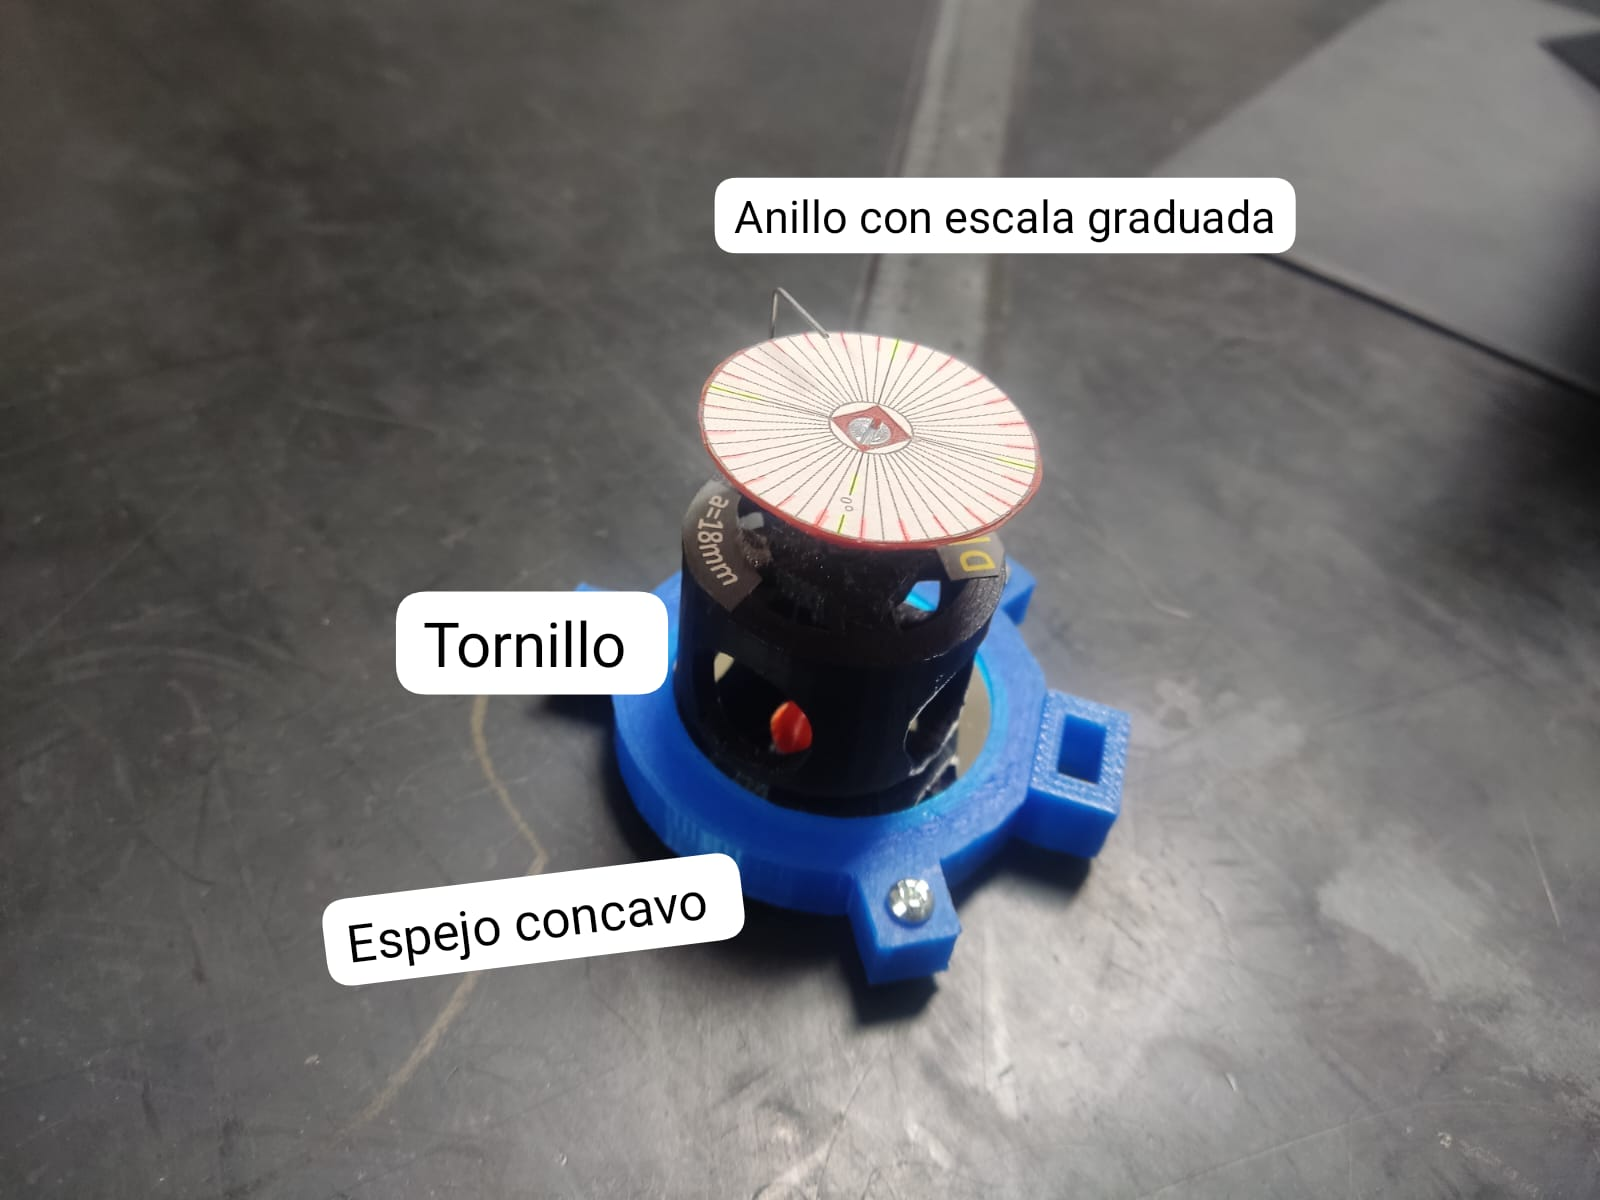
\includegraphics[width=0.5\linewidth]{esferometro arreglo.jpeg}
    \caption{Arreglo experimental esferómetro}
    \label{fig:enter-label}
\end{figure}

\subsection{Medición de la Distancia Imagen y Comparación de Magnificaciones}
Para comprobar experimentalmente la ecuación del espejo cóncavo, se implementó un montaje experimental similar al de la Figura 5 del documento de referencia. El procedimiento fue el siguiente:

\begin{enumerate}
    \item Se colocó un espejo cóncavo en una base fija, alineando su vértice con el punto cero de una escala de medición.
    \item A un lado de la escala se ubicó una pantalla para proyectar la imagen reflejada, y al otro lado se colocó un objeto luminoso (por ejemplo, una lámpara). Tanto la pantalla como el objeto se colocaron sobre bases móviles.
    \item Se ajustó la altura de los tres elementos (espejo, pantalla y objeto) para asegurar que estuvieran alineados con el eje óptico del espejo y minimizar distorsiones.
    \item Se variaron las posiciones del objeto a lo largo de la escala, registrando para cada posición la distancia imagen correspondiente proyectada en la pantalla.
    \item Se midieron las alturas del objeto ($h$) y de la imagen proyectada ($h'$) para cada par de distancias objeto-imagen $(o, i)$.
    \item Se calculó el foco del espejo utilizando la ecuación del espejo:
    \begin{equation}
        \frac{1}{o} + \frac{1}{i} = \frac{1}{f}
    \end{equation}
    \item Se verificó la relación de magnificación mediante la ecuación:
    \begin{equation}
        M = \frac{h'}{h} = -\frac{i}{o}
    \end{equation}
\end{enumerate}

Este procedimiento permitió obtener experimentalmente el foco del espejo cóncavo y validar la ecuación de la magnificación comparando el tamaño del objeto y la imagen proyectada en la pantalla.

\begin{figure}[H]
    \centering
    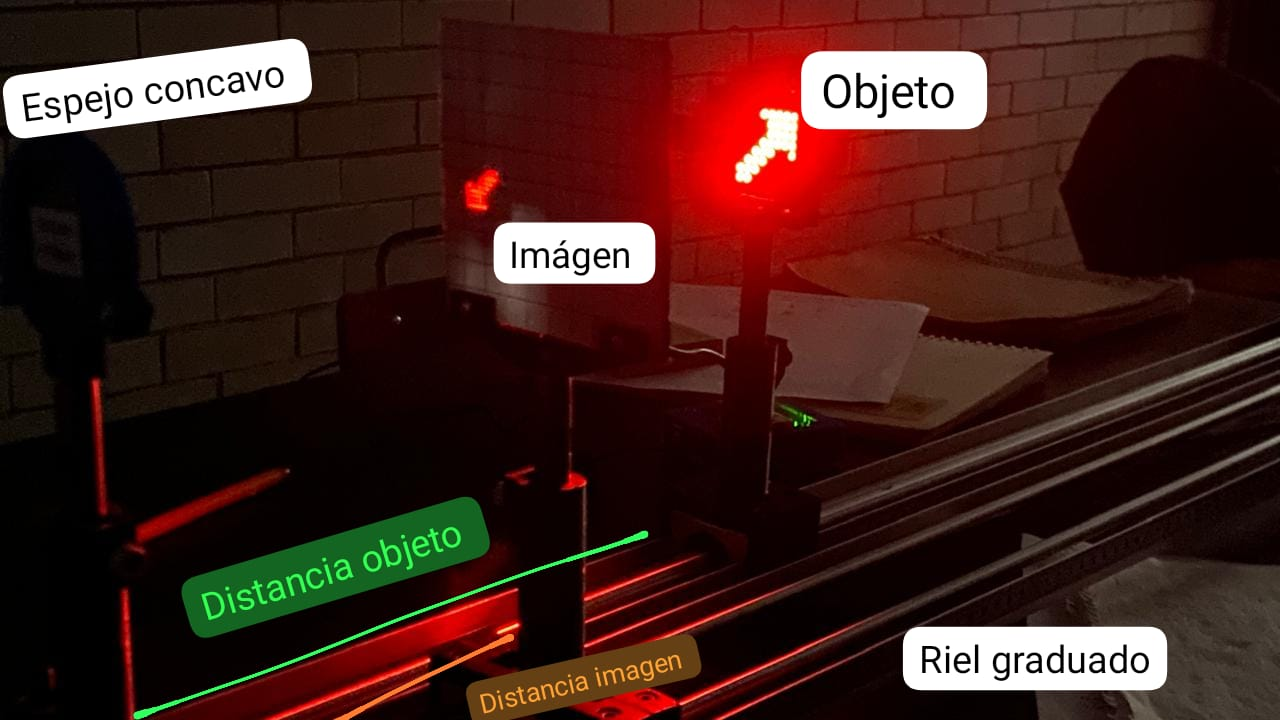
\includegraphics[width=0.5\linewidth]{espejo concavo arreglo.jpeg}
    \caption{Arreglo experimental para el espejo esférico}
    \label{fig:enter-label}
\end{figure}



\section{Resultados y discusión del tratamiento de datos}

\subsection{Espejo Plano}
Tras hacer el procedimiento de triangulación obtenemos que nuestra distancia imagen es $(4.76 \pm 0.41)cm$, recordemos que nuestra distancia objeto era de 5cm, por lo que este resultado si bien nos da indicio de que la ley de reflexión preserva distancias $s_i=s_o$, el resultado no es tan contundente y podemos incluso asociar magnificación transversal al espejo plano en este margen de incertidumbre. Sugerimos para siguientes estudios usar distancias mucho más grandes y más líneas para la triangulación.

\subsection{Esferometro}

\begin{table}[H]
\centering
\begin{tabular}{cccccccc}
\rowcolor[HTML]{C0C0C0} 
\textbf{a [mm]} & \textbf{$\Delta a$ [mm]} & \textbf{h [mm]} & \textbf{$\Delta$h [mm]} & \textbf{Radio [
Cm]} & \textbf{$\Delta$Radio [Cm]}& f [cm]& $\Delta F$ [CM] \\ 
\hline
\rowcolor[HTML]{DAE3F3} 18 & 0.210 & 0.806 & 0.025 & 20.14 & 0.7 & 10.07 & 0.4 \\ 
\hline
\end{tabular}
\caption{Mediciones obtenidas con el esferómetro}
\label{tab:esferometro}
\end{table}

Para esta etapa del experimento como puede usted lector apreciar en la tabla, se ha registrado la distancia de desplazamiento vertical así como se ha medido la distancia horizontal del tornillo central del esferómetro a una de las patas externas. Aplicando la ecuación mostrada en el marco teórico (Eq. 5). Se tiene en consecuencia que el radio de curvatura del espejo esférico es de $(20.1\pm0.7)cm$, en tanto que la distancia focal es de $(10.0 \pm 0.4)cm$.


\subsection{Espejo Concavo}
(Puede consultar la tabla relacionada a este experimento en el siguiente enlace \cite{Excel})

Para este espejo, al graficar distancia objeto vs distancia imagen obtenemos el siguiente gráfico.
\begin{figure}[H]
  \centering
    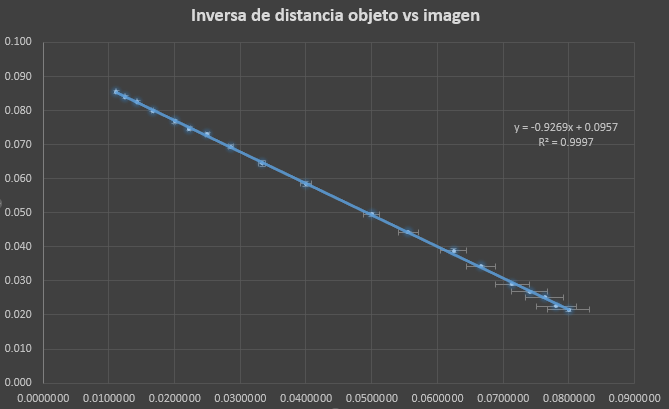
\includegraphics[width=0.6\linewidth]{concavo2.png}
    \caption{Regresión lineal aplicada a $s_0^{-1} \textit{ vs } s_i^{-1}$}.
    \label{fig:enter-label}
\end{figure}
De aquí, nótese que si bien parece tener un comportamiento semejante a un exponente $-0.673$, la $R^2$ de este gráfico deja mucho de qué desear. Probablemente existe un desfase que provoca que el gráfico no viva centrado en el origen como nos parecería. Véase a continuación el siguiente gráfico de los inversos de la distancia objeto vs distancia imagen.


En esta ocasión la recta es quasiperfecta, además, el coeficiente de Pearson $R^2$ es demasiado semejante al 1, por lo que este gráfico efectivamente presentaba un pequeño desfase respecto al origen, algo que el gráfico anterior carecía en su información pues la regresión potencial no es capaz de considerar estos desplazamientos. Por lo cual, tenemos la siguiente expresión.
\begin{equation}
    s_i^{-1} = -(0.9269\pm0.0039)s_o^{-1} + (0.0957 \pm 0.0002)
\end{equation}
La teoría nos indica que en realidad, el gráfico debería comportarse como $s_0^{-1} + 2R^{-1} = s_{i}^{-1}$. Véase que esto se obtendría si se considera la ordenada al origen como $2R^{-1}$. Por lo que se obtiene que $R = 2(0.0957)^{-1}cm = 20.90 cm$ y su incertidumbre estara dada por la suma en cuadratura de la nominal (Ec.15) y la estadistica, por tanto $R=20.90 \pm 0.44cm $ y foco es $f=10 \pm 0.22$

\subsection{Comparación de los Radios}

Del procedimiento con el esferómetro tenemos que el radio del espejo esférico es de $(20.14 \pm 0.70)cm$, en tanto que en este resultado previo obtuvimos que $R=(20.90 \pm 0.44)$cm; no podemos atribuir un resultado definitivo pues si bien el espejo ya indicaba que el radio de curvatura es de 20cm, desconocemos los desperfectos que el fabricante ha reportado en su fabricación, por lo cual su radio verdadero podría incluso estar centrado en estos dos valores. Si bien el resultado obtenido por el esferómetro parece más exacto no es tan preciso, pues manipular magnitudes tan pequeñas que al manipularse en la ecuación los errores pueden hacerse macroscópicos nos da un margen de incertidumbre muy amplio. Mientras que el método de mapeo distancia objeto vs distancia imagen reporta un dato aparentemente menos exacto pero con un muy alto índice de precisión.

\subsection{Magnificación}

Al acercar el objeto al espejo (aumento de \( o \) de \( 12.50\ \text{cm} \) a \( 13.50\ \text{cm} \)), la posición de la imagen (\( i \)) disminuye de \( 44.00\ \text{cm} \) a \( 37.30\ \text{cm} \), y la altura de la imagen (\( h' \)) se reduce de \( 6.75\ \text{cm} \) a \( 5.20\ \text{cm} \). Esto resulta en una disminución de la magnificación transversal (\( M \)) de \( 3.534 \) a \( 2.723 \), indicando que la imagen se hace más pequeña respecto al objeto conforme el objeto se aproxima al espejo.  \\
Para un espejo cóncavo, la magnificación teórica se expresa como \( M = -\frac{i}{o} \), donde el signo negativo indica inversión de la imagen. Sin embargo, en este caso, las imágenes son derechas (no invertidas), lo que sugiere que el objeto se encuentra dentro de la distancia focal del espejo, generando imágenes virtuales. Los valores experimentales de \( M \) son consistentes con este comportamiento: al estar el objeto cerca del espejo, la imagen virtual es amplificada pero disminuye en tamaño relativo al aumentar \( o \). 

\begin{figure}[H]
    \centering
    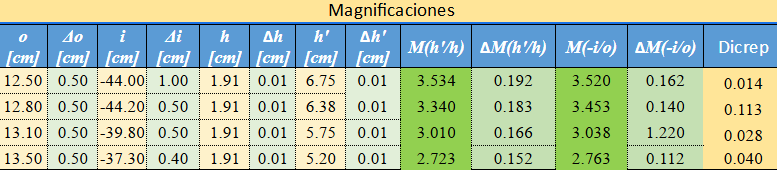
\includegraphics[width=0.65\linewidth]{Magnificación.png}
    \caption{Tabla de magnificación tabla obtenida de: \cite{Excel}}
    \label{fig:enter-label}
\end{figure}

De la tabla de maginificación podemos observar que la discrepancia entre $M(h/h´)$ y $M(-i/o)$ es menor que sus incertidumbres  para cada una de las posiciones, por lo tanto podemos concluir que ambas formulas son validas. 

\section{Conclusiones}

A partir de los experimentos realizados con espejos planos y cóncavos, se concluye lo siguiente:

La distancia imagen en un espejo plano es my similar a la distancia objeto, validando la ley de reflexión.

La medición del radio de curvatura del espejo cóncavo con el esferómetro resultó consistente con la obtenida mediante la ecuación del espejo.

Se verificó la relación de magnificación, observándose que el tamaño de la imagen se relaciona con la distancia del objeto al espejo de acuerdo con la ecuación teórica.
 
El análisis gráfico de la ecuación del espejo permitió obtener experimentalmente el valor del foco, confirmando la validez del modelo óptico.

El experimento demostró la validez de las ecuaciones ópticas para la formación de imágenes en espejos planos y esféricos. Se encontraron diferencias mínimas entre los valores experimentales y los teóricos, lo que resalta la precisión del método empleado. La propagación de incertidumbre sugiere que el método de linealización de la ecuación del espejo puede ser una alternativa confiable para determinar el radio de curvatura.
 



\begin{thebibliography}{9}

\begin{thebibliography}{99}
    \bibitem{Pedrotti2018} F. L. Pedrotti, L. M. Pedrotti, L. S. Pedrotti, \textit{Introduction to Optics}, Cambridge University Press, 2018, 3° ed.
    \bibitem{Hecht2000} E. Hecht, \textit{Óptica}, 3° edición, Addison Wesley, 2000.
    \bibitem{Tipler1999} P. A. Tipler, \textit{Physics for Scientists and Engineers}, 4° edición, Freeman/Worth, 1999.
    \bibitem{Serway2002} R. A. Serway, R. J. Beichner, \textit{Física para Ciencias e Ingeniería}, 5° edición, McGraw-Hill, 2002.
    \bibitem{Khan2015} S. A. Khan, \textit{Coordinate Geometric Generalization of the Spherometer and Cylindrometer}, arXiv:1311.3602, 2015.
    \bibitem[]{Excel} A. Reyes, S. Tablas de Reflexión y Refracción, Archivo Excel. 2024. Disponible en: \href{https://docs.google.com/spreadsheets/d/14DnqcfldTRxWjrozeFOlHG4xXEaZAA9k/edit?usp=sharing\&ouid=112625838925660900694\&rtpof=true\&sd=true}{Enlace al documento}
\end{thebibliography}

\end{thebibliography}


\section*{Apéndice: Propagación de incertidumbre}

\subsection*{Incertidumbre del radio de curvatura}
A partir de la ecuacion de espejos :

\begin{mdframed}
\begin{equation}
    R = 2\left(\frac{o i}{o + i}\right)
\end{equation}
\end{mdframed}
Usamos la regla de propagación de errores:
\begin{mdframed}
\begin{equation}
    (\sigma_R)^2 = \left( \frac{2i^2}{(o + i)^2} \sigma_o \right)^2 + \left( \frac{2o^2}{(o + i)^2} \sigma_i \right)^2
\end{equation}
\end{mdframed}
\subsection*{Incertidumbre del foco}
La relación entre el radio de curvatura y la distancia focal es:

\begin{mdframed}
\begin{equation}
    f=\frac{R}{2}
\end{equation}
\end{mdframed}

Por lo que su incertidumbre será

\begin{mdframed}
\begin{equation}
    \sigma _f=\frac{\sigma _R}{2}
\end{equation}
\end{mdframed}

\subsection*{Incertidumbre de la magnificación}
La magnificación está dada por:
\begin{mdframed}
\begin{equation}
    M = -\frac{i}{o}
\end{equation}
\end{mdframed}

Aplicamos la propagación de incertidumbre:
\begin{mdframed}
\begin{equation}
    \sigma_M^2 = \left( \frac{\partial M}{\partial i} \sigma_i \right)^2 + \left( \frac{\partial M}{\partial o} \sigma_o \right)^2
\end{equation}
\end{mdframed}
Calculamos las derivadas:
\begin{mdframed}
\begin{equation}
    \frac{\partial M}{\partial i} = -\frac{1}{o}, \quad \frac{\partial M}{\partial o} = \frac{i}{o^2}
\end{equation}
\end{mdframed}
Sustituyendo:
\begin{mdframed}
\begin{equation}
    \sigma_M = \frac{1}{o} \sqrt{\sigma_i^2 + \left(\frac{i}{o} \sigma_o\right)^2}
\end{equation}
\end{mdframed}

\subsection*{Incertidumbre en términos de $h_i$ y $h_o$}
También se puede expresar como:
\begin{mdframed}
\begin{equation}
    M = \frac{h_i}{h_o}
\end{equation}
\end{mdframed}
Aplicamos la propagación de incertidumbre:
\begin{mdframed}
\begin{equation}
    \sigma_M^2 = \left( \frac{\partial M}{\partial h_i} \sigma_{h_i} \right)^2 + \left( \frac{\partial M}{\partial h_o} \sigma_{h_o} \right)^2
\end{equation}
\end{mdframed}
Derivamos:

\begin{mdframed}
\begin{equation}
    \frac{\partial M}{\partial h_i} = \frac{1}{h_o}, \quad \frac{\partial M}{\partial h_o} = -\frac{h_i}{h_o^2}
\end{equation}
\end{mdframed}

Sustituyendo:
\begin{mdframed}
\begin{equation}
    \sigma_M = \frac{1}{h_o} \sqrt{\sigma_{h_i}^2 + \left(\frac{h_i}{h_o} \sigma_{h_o}\right)^2}
\end{equation}
\end{mdframed}

\subsection*{Incertidumbre del radio de curvatura}
A partir del esferometro, sabemos que:

\begin{mdframed}
\begin{equation}
    R = \frac{a^2}{2h} + \frac{h}{2}
\end{equation}
\end{mdframed}

Aplicamos la prpagación de incertidumbre:

\begin{mdframed}
\begin{equation}
    \sigma_R^2 = \left( \frac{\partial R}{\partial a} \sigma_{a} \right)^2 + \left( \frac{\partial R}{\partial h} \sigma_{h} \right)^2
\end{equation}
\end{mdframed}

Derivamos:

\begin{mdframed}
\begin{equation}
    \frac{\partial R}{\partial a} = \frac{a}{h}, \quad \frac{\partial R}{\partial h} = -\frac{h^2-a^2}{2h^2}
\end{equation}
\end{mdframed}

Sustituyendo:

\begin{mdframed}
\begin{equation}
    \sigma_R = \sqrt{\left(\frac{a}{h}\sigma_{a}\right)^2 + \left(\frac{h^2-a^2}{2h} \sigma_{h}\right)^2}
\end{equation}
\end{mdframed}

\end{document}